\chapter{Análisis y Diseño}
En este capítulo se presenta el modelo del dominio, el modelo conceptual y el modelo físico en su versión final. Posteriormente se describe la estructura y se desarrolla cada casos de uso de acuerdo a ICONIX.
\begin{landscape}
\section{Modelo del Dominio}
    \begin{figure}[H]
        \centering
        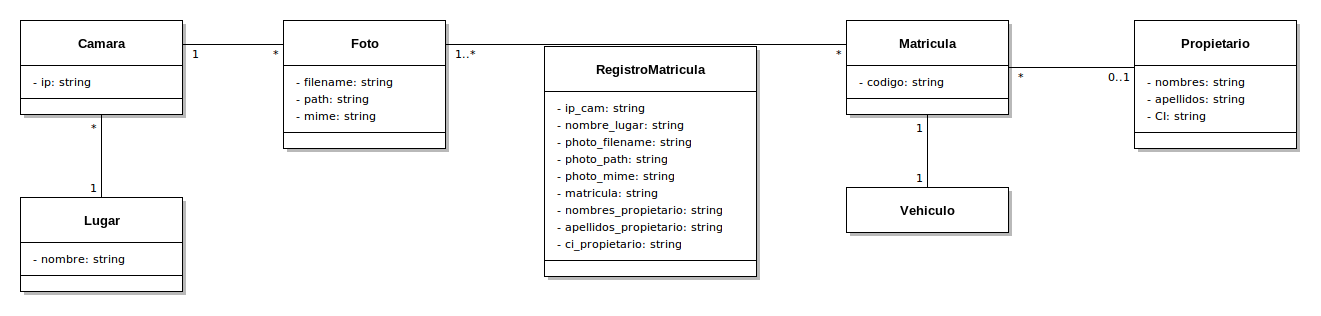
\includegraphics[width=1.3\textwidth]{DOM}
        \caption{Modelo del Dominio}
        \label{fig:DOM}
    \end{figure}
\end{landscape}

\newpage 
\eject \pdfpagewidth=420mm \pdfpageheight=297mm
\section{Modelo Conceptual}
    \begin{figure}[H]
        \centering
        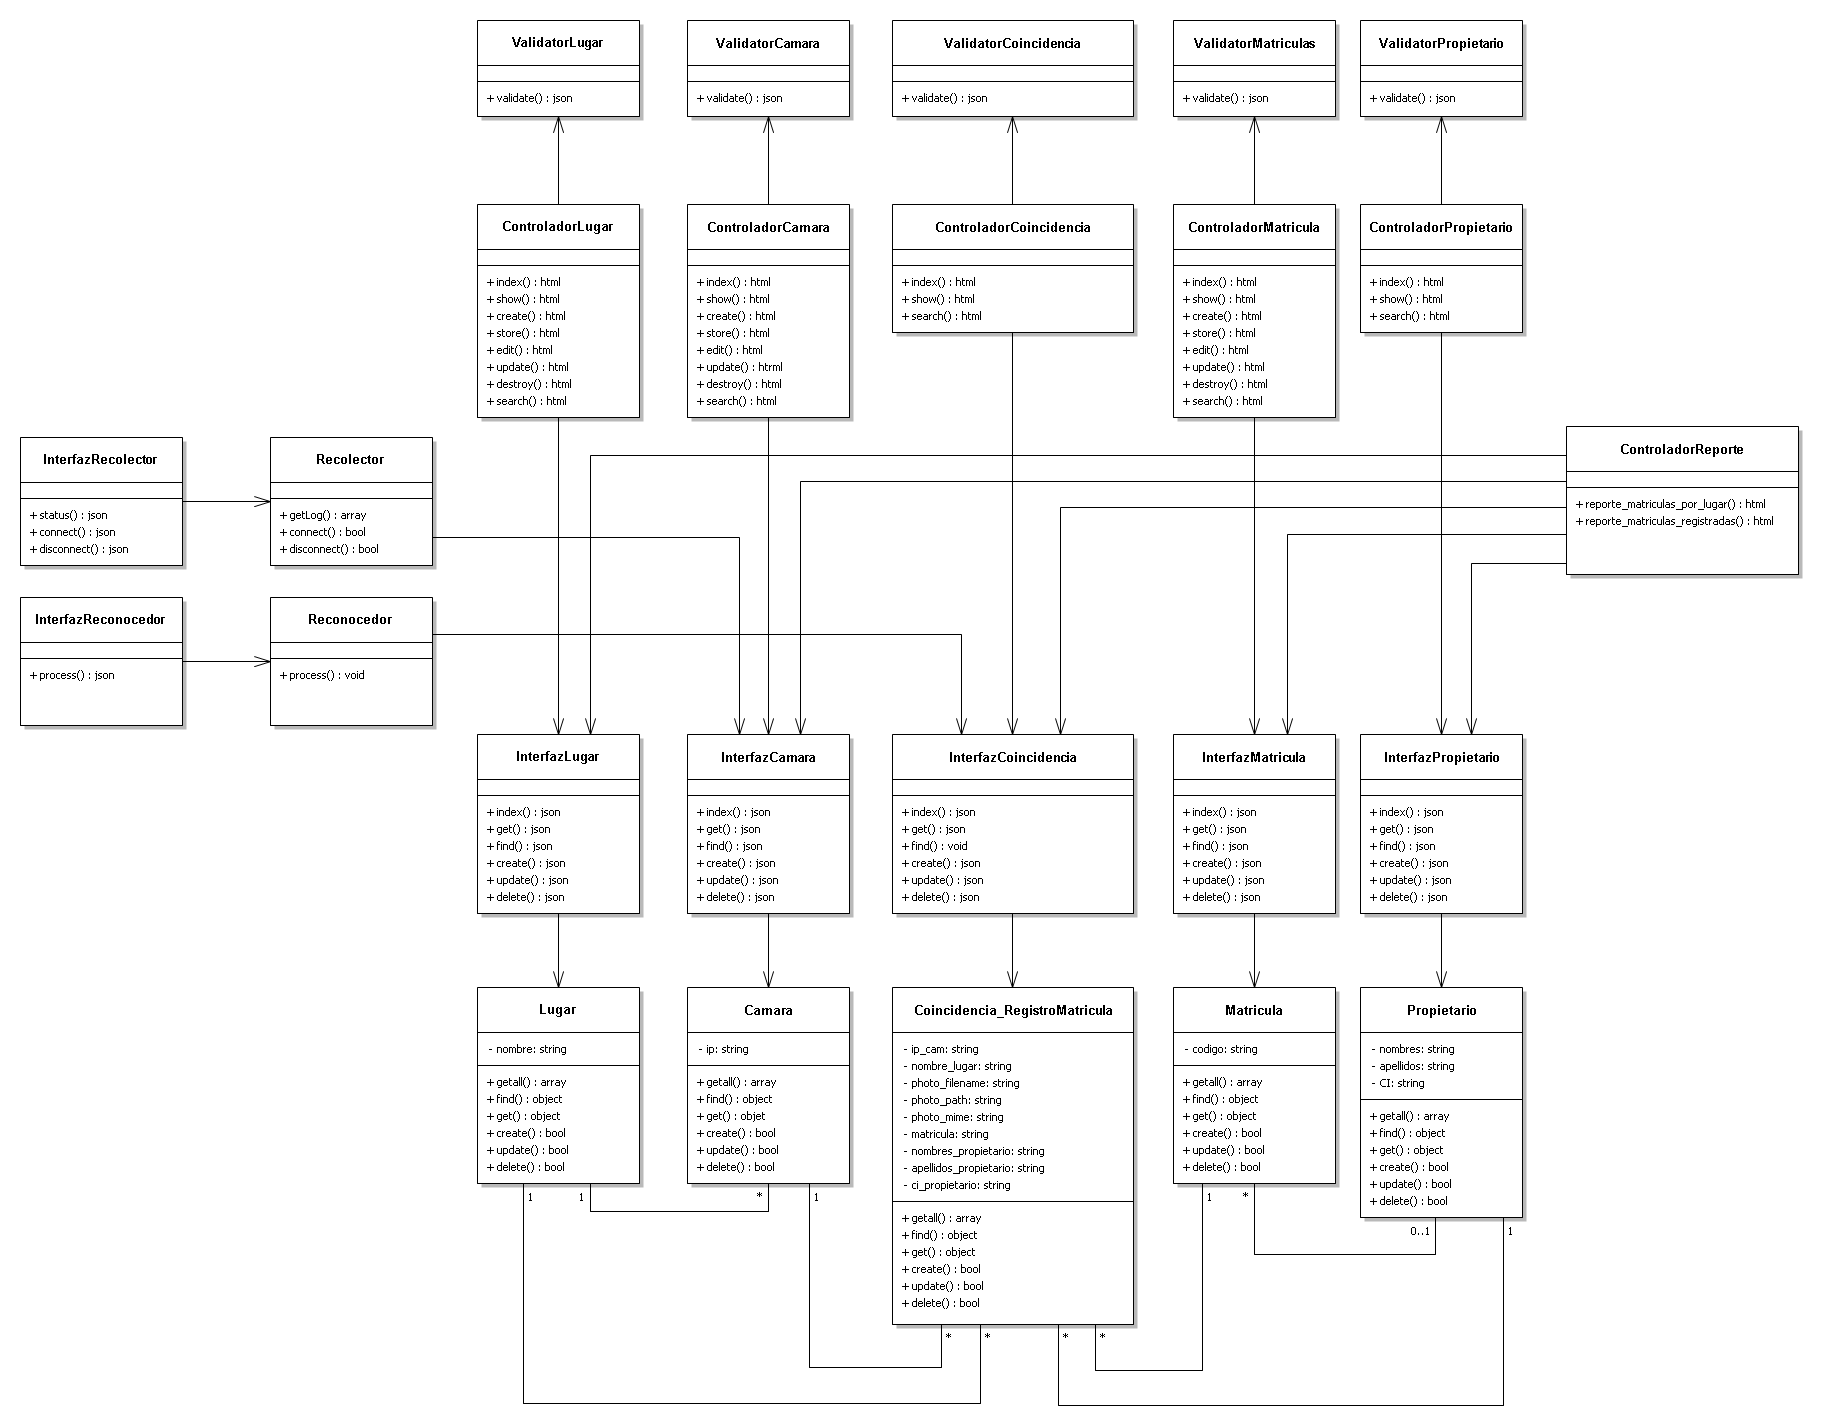
\includegraphics[width=1.3\textwidth]{CLASS}
        \caption{Modelo Conceptual}
        \label{fig:CLASS}
    \end{figure}

\newpage
\eject \pdfpagewidth=215.9mm \pdfpageheight=279.4mm
 
\section{Modelo Físico}
    \begin{figure}[H]
        \centering
        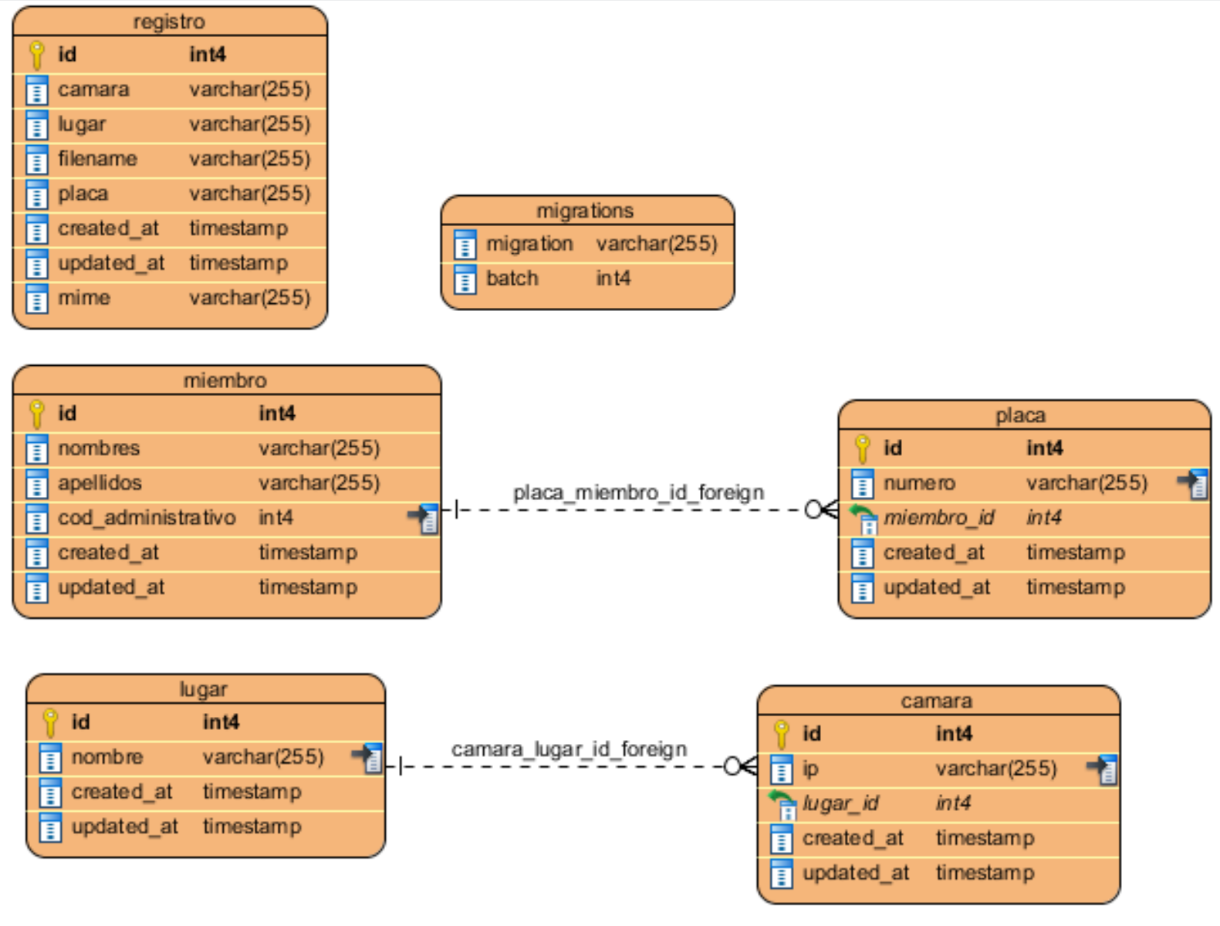
\includegraphics[width=.9\textwidth]{FISICO}
        \caption{Modelo Físico}
        \label{fig:FISICO}
    \end{figure}


\section{Estructura ICONIX para los Casos de Uso}
La descripción de cada caso de uso, de acuerdo con ICONIX, debe seguir la siguiente estructura: 
\begin{itemize}
    \item Descripción del Caso de Uso
    \item Diagrama de Caso de Uso
    \item Interfaz Gráfica Tentativa
    \item Diagrama de Robustez
    \item Diagrama de Secuencia
\end{itemize}
